\scanpage{51}
\mspage{\handwritten{19}}
% archive sheet number: 50

\deleted{ouvert (EGA IV 2.4.9), il \deleted{pas} suffit de prouver qu'i\deleted{\unsure{o|h}}\inserted{l} existe une telle extension $k'$ et un point $x'$ de $H'=H\otimes_k k'$ au dessus de $x$, tels que $H'-G'$ soit un voisinage de $x'$. Or \deleted{on}\handwritten{il} suffira de prendre \deleted{$k$} $k'=k(x)$, de sorte que $G'$ admet un point $x'$ rationnel sur $k'$ au dessus de $x$. Alors l'ouvert dans $H'$ translaté de $G'$ par $x'$ contient $x'$ et est contenu dans $H'-G'$\handwritten{,}\deleted{\unsure{qui}} qui est donc un voisinage de $x'$, ce qui achève la démonstration de 11.11.}

\uline{Remarque} 11.11.\deleted{\unsure{3|1}}\handwritten{1}. \deleted{Monsieur} M. Raynaud nous signale qu'on peut générali-\linebreak ser 11.11 au cas d'un schéma en groupes quasi-compact et quasi-s\deleted{p}\handwritten{é}\deleted{\unsure{é|e}}\handwritten{p}aré $G$ sur un schéma\inserted{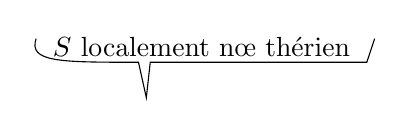
\begin{tikzpicture}[x=1cm,y=1cm,baseline=(n.base)]\node (n) at (0,0) {$S$ localement n\oe{} thérien};\draw (-2.1,.1) .. controls (-2.2,-.2) and (-1.8,-.2) .. (-.8,-.2)--(-.7,-.65)--(-.65,-.2)--(2.1,-.2)--(2.2,.1);\end{tikzpicture}} régulier de dimension $\handwritten{\leqslant}1$, en supposant de plus $G$ \uline{plat} sur $S$. 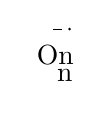
\begin{tikzpicture}[x=1cm,y=1cm,baseline=(n.base)]\node (n) at (0,0) {On};\node at (.12,-.26) {\handwritten{n}};\draw (-.03,.33)--(.08,.33);\fill (.18,.33) circle (.018);\end{tikzpicture} a alors équivalence des conditions suivantes:

(i) $G$ est affine sur $S$.

(ii) $G$ est quasi-affine sur $S$.

(iii) \unsure{G|O}n peut faire opérer $G$ fidèlement sur un $S$-schéma quasi-affine.

(iv) On peut faire opérer $G$ fidèlement sur un Module quasi-cohérent plat sur $S$.

(v) (Si $G$ est de type fini sur $S$\inserted{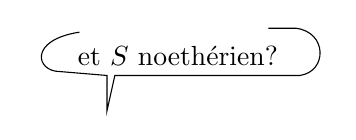
\begin{tikzpicture}[x=1cm,y=1cm,baseline=(n.base)]\node (n) at (0,0) {et $S$ noethérien\handwritten{?}};\draw (-1.25,.3) .. controls (-1.9,.2) and (-1.8,-.2) .. (-1.5,-.2)--(-.9,-.25)--(-.9,-.7)--(-.8,-.25)--(1.55,-.25) .. controls (1.9,-.2) and (1.9,.3) .. (1.5,.35)--(1.15,.35);\end{tikzpicture}}) $G$ est isomorphe à un sous-groupe fermé d'un $\text{\uline{Aut}}_V$, où $V$ est un Module localement libre de type fini sur $\handwritten{\unsure{\mathbb{S}|S}}$.

% Handwritten relocation arrow, from the lower remark towards the upper remark.
\margin{\figure{\handwritten{\begin{tikzpicture}[x=0.35cm,y=0.35cm]\draw (1,0) .. controls (0.1,-0.3) and (0.1,0.1) .. (0.1,0.7) -- (0.1,2) .. controls (0.1,2.7) and (0.4,2.8) .. (1,2.8);\draw (0.2,2.5) .. controls (-.6,3.5) and (-.7,6.2) .. (-.9,8.0);\draw[->] (-.92,8.15) .. controls (-.97,9.3) and (-1,10.5) .. (-.8,11) .. controls (-.4,12) and (0.5,12.4) .. (1.6,12.5);\end{tikzpicture}}}}
\deleted{\uline{Remarque} 11.11.2. Avec les notations de la démonstration précédente, on voit facilement (une fois qu'on sait que $G$ est affine) que \unsure{G'|l'}homomor-\linebreak phisme $G\handwritten{\longrightarrow}G'=\underset{\handwritten{\longleftarrow}}{\lim}G_i$ est un isomorphisme, ce qui donne pour $G$ un théorème de structure\handwritten{,} qui sera \deleted{repris}\inserted{prouvé} par une autre méthode dans 11.1\deleted{\unsure{3}}\handwritten{5}.}
